% ******************************* Thesis Appendix A ****************************
\chapter{The code and inputs}

\section{Building the dislocation}
\label{sec:building_disloc_code}

Given below are a set of python functions to build an array of atoms in the form described in \autoref{sec:build}. Also defined are some example inputs such as the input for the NaCl slip systems.
 Typical use would be to import this as a module to a script and use the first three functions.
 
 
\lstinputlisting{Appendix_1/build.py}

\section{Inputs}
\label{sec:pyerls_inputs}

\subsection{Elastic Tensors for cementite under different levels of hydrogen loading.}



\section{Analysing the results}
\label{sec:analysing_results_code}

\section{Ionic energy calculations}
\label{sec:ionic_energy_code}
%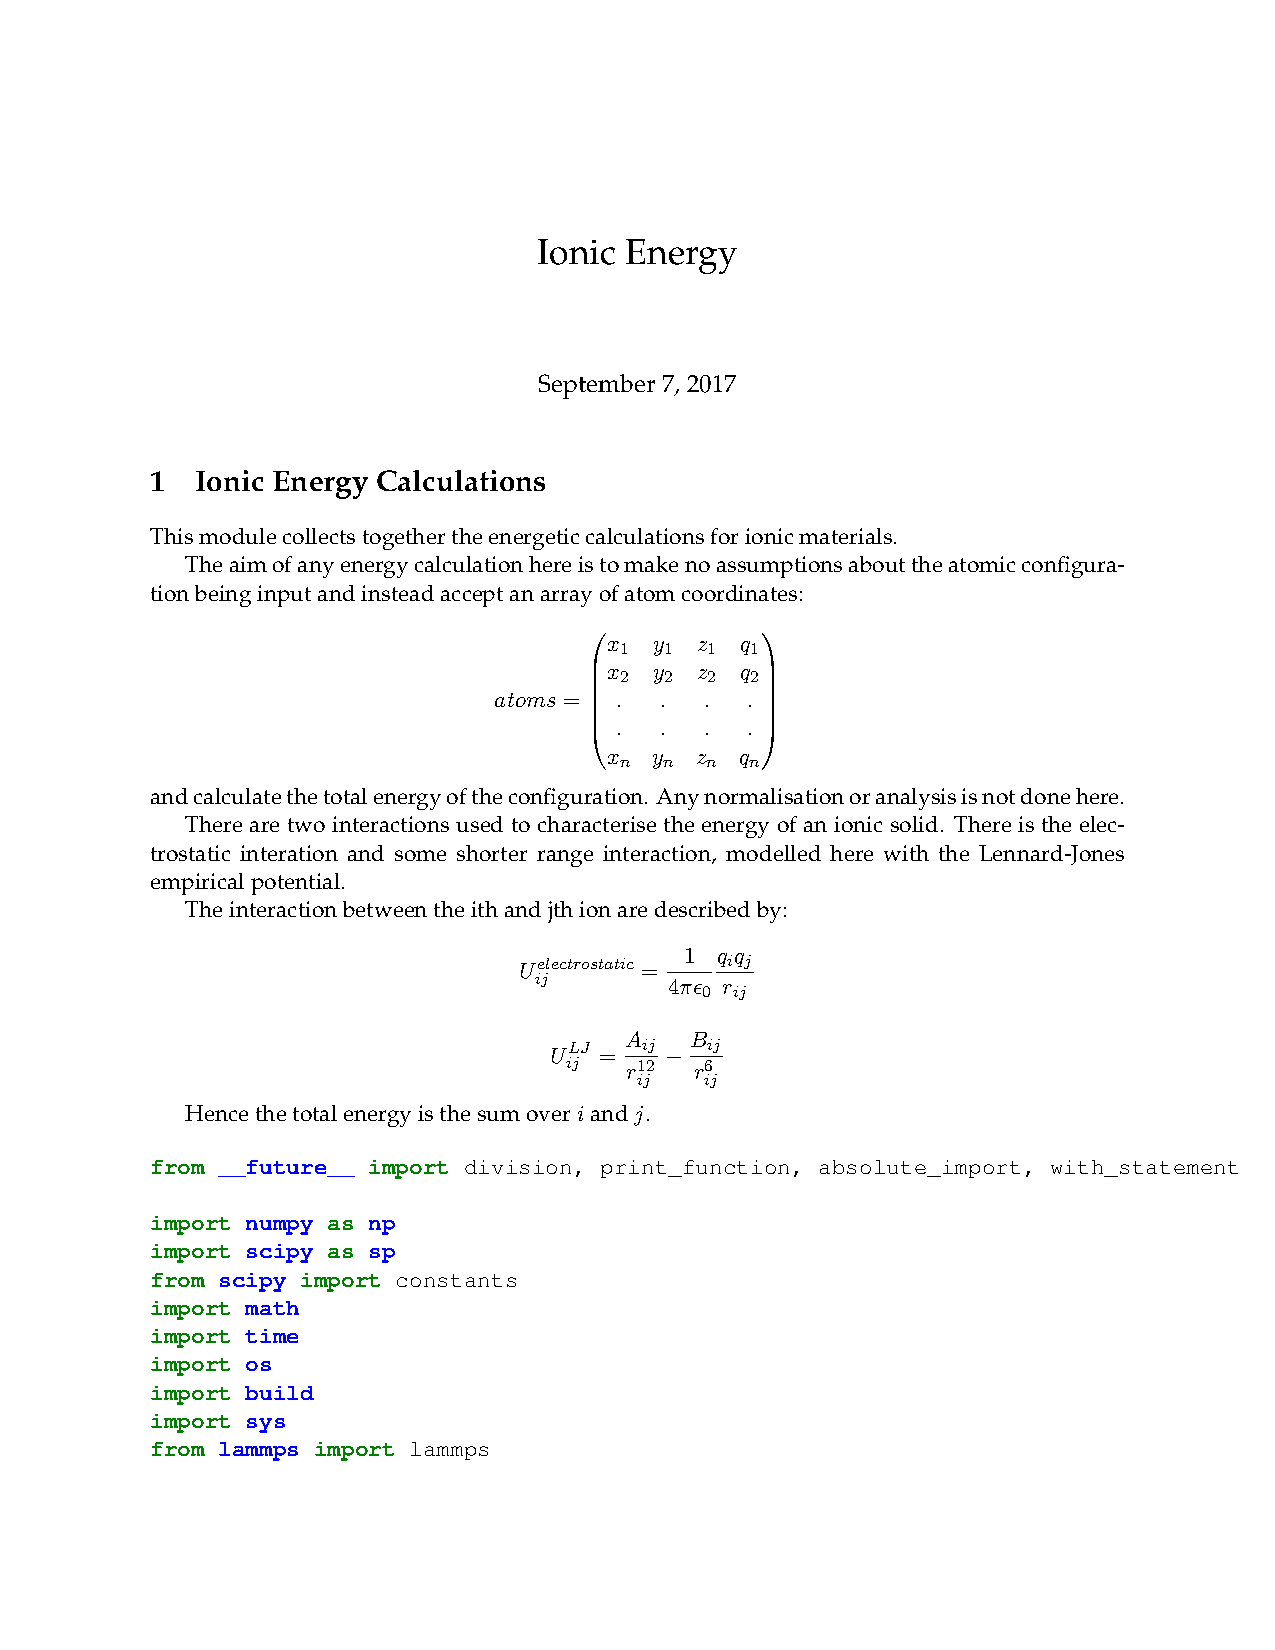
\includepdf[pages=-]{Appendix1/ionic-energy.pdf}


\section{LAMMPS inputs}
\label{sec:lammps_input}
